\section{General}
The software has the task to gather the image information from the camera, detecting the ball, predicting where it will go in the future and controlling the motors to either stop or shoot the ball.
This task can be split into the following chapters:
\begin{itemize}
    \item \textbf{Optics}: Correcting for Lens distortion
    \item \textbf{Ball Detection}: Detecting the ball in the image and converting the coordinates to real world coordinates
    \item \textbf{Prediction}: Predicting the ball movement
    \item \textbf{Controlling the motors}: Finally, we move the motors to the correct position
\end{itemize}

\section{Optics}
The goal here is to correct for lens distortion, this can be achieved by first capturing many images containing a checkerboard pattern with known gird size, in this is case 8x8.
One such image in my case looks like this:\begin{figure}[H]
    \centering
    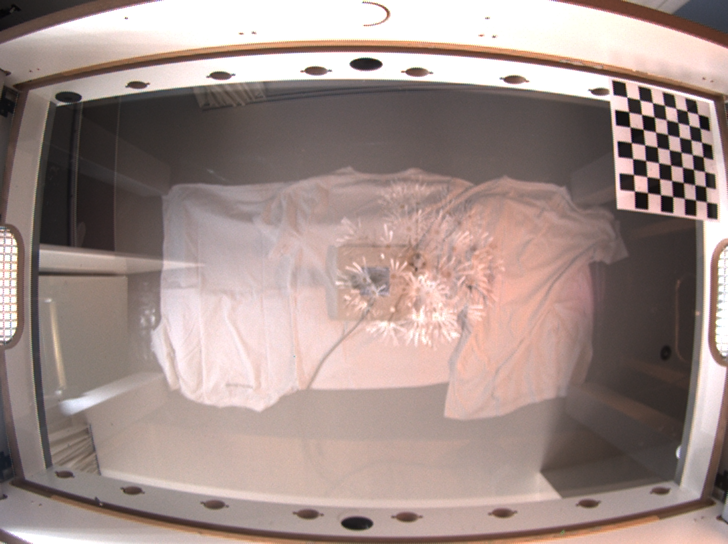
\includegraphics[height=5cm]{../photos/calibration_image}
    \caption[calimage]{Calibration image}
    \label{fig:calibration_image}
\end{figure}
As one can see there is severe distortion in the image, this can be corrected by using the OpenCV library.
